\documentclass[14pt]{extarticle}
\usepackage[utf8]{inputenc}
\usepackage[T1]{fontenc}
\usepackage[spanish,es-lcroman]{babel}
\usepackage{amsmath}
\usepackage{amsthm}
\usepackage{physics}
\usepackage{tikz}
\usepackage{float}
\usepackage[autostyle,spanish=mexican]{csquotes}
\usepackage[per-mode=symbol]{siunitx}
\usepackage{gensymb}
\usepackage{multicol}
\usepackage{enumitem}
\usepackage[left=2.00cm, right=2.00cm, top=2.00cm, 
     bottom=2.00cm]{geometry}

%\renewcommand{\questionlabel}{\thequestion)}
\decimalpoint
\sisetup{bracket-numbers = false}

\title{\vspace*{-2cm} Práctica 2 - Sonido y distancia \\  Reporte - Física IV (Área II) \vspace{-5ex}}
\date{}

\begin{document}
\maketitle
\

\section{Discusión de resultados y conclusiones.}

En este apartado deberás de responder las siguientes preguntas:
\begin{enumerate}
\item Con mis datos experimentales: ¿se aprecia una tendencia de tipo hiperbólico (es decir, una tendencia del tipo $\dfrac{1}{r^{2}}$)? Si tu respuesta es Si/No, deberás de explicar el por qué.
\item ¿Consideras que se necesitan más datos experimentales para que se aprecie mejor la tendencia de respuesta entre la Intensidad de sonido y la distancia de la fuente? ¿Por qué?
\item Al utilizar un sonómetro de aplicación del equipo celular, ¿es confiable su uso para uso en un laboratorio? justifica tu respuesta.
\end{enumerate}

Con los siguientes datos construye una gráfica de Intensidad de sonido (eje y, con unidades \unit{\watt\per\square\meter}) y distancia (eje x con unidades \unit{\meter}), procura ajustar la escala para que se aproveche al máximo la curva obtenida.
\begin{table}[H]
\centering
\begin{tabular}{| c | c | c | c | c | c | c | c | c | c | c |} \hline
Eje x & $1$ & $2$ & $3$ & $4$ & $5$ & $6$ & $7$ & $8$ & $9$ & $10$ \\ \hline
Eje y & $1$ & $0.25$ & $0.11$ & $0.0625$ & $0.04$ & $0.027$ & $0.02040$ & $0.0156$ & $0.01234$ & $0.01$ \\ \hline
\end{tabular}
\end{table}
Te puedes apoyar con un programa informático, tipo Excel para generar una gráfica, que sería como la que se muestra a continuación:
\begin{figure}[H]
     \centering
     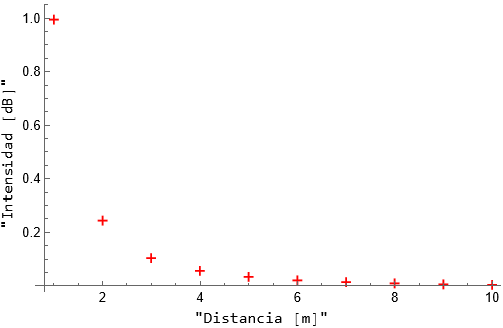
\includegraphics[scale=0.8]{Imagenes/Cuadrado_inverso_01.png}
     \caption{Datos experimentales.}
\end{figure}
Se aprecia una tendencia en los datos, por lo que el siguiente paso es iniciar una aproximación, la más básica es con una línea recta, como se ve en la siguiente figura:
\begin{figure}[H]
     \centering
     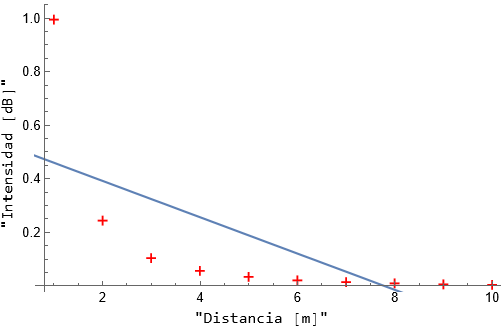
\includegraphics[scale=0.8]{Imagenes/Cuadrado_inverso_02.png}
     \caption{Ajuste lineal en los datos.}
\end{figure}
Vemos de la figura anterior que los datos no se ajustan con la línea recta, por lo que debemos de realizar un ajuste cuadrático, es decir con una potencia de $d^{2}$ en el eje de las abscisas, el eje horizontal:
\begin{figure}[H]
     \centering
     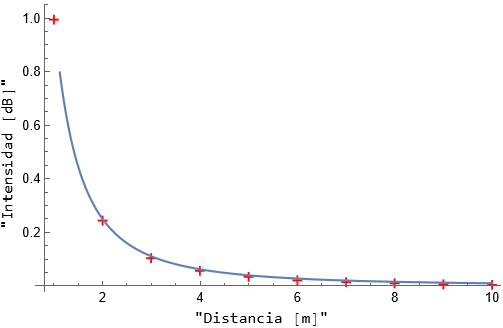
\includegraphics[scale=0.8]{Imagenes/Cuadrado_inverso_03.png}
     \caption{Ajuste cuadrático en los datos.}
\end{figure}
Ahora encontramos que el ajuste es más directo y que pasa prácticamente por todos los puntos experimentales. Hasta este punto, podemos decir que la relación entre la intensidad de sonido y la distancia es del tipo:
\begin{align*}
I \propto \dfrac{1}{d^{2}}
\end{align*}
Para estimar el exponente de la relación, se hace un cambio en los ejes de la gráfica, pasamos de una escala lineal a una escala logarítmica en ambos ejes, conocida como escala log-log, de tal manera que tendremos:
\begin{figure}[H]
     \centering
     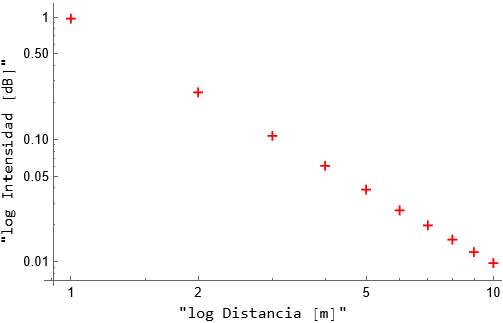
\includegraphics[scale=0.8]{Imagenes/Cuadrado_inverso_04.png}
     \caption{Cambio a un eje log-log en las coordenadas de la gráfica.}
\end{figure}
La pendiente de la recta que vemos es la tendencia de los datos, correspondería al exponente $-2$. Con Excel intenta modificar los ejes x-y de la gráfica. 
\end{document}